9. \begin{figure}[ht!]
\center{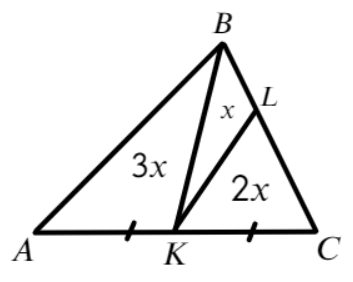
\includegraphics[scale=0.35]{g9-9.png}}
\end{figure}\\
Если треугольники имеют общую высоту, их площади относятся так же, как основания, к которым проведена эта высота. Поэтому $S_{\Delta BLK}=x,\ S_{\Delta KLC}=2x,$ а $S_{\Delta ABK}=S_{\Delta BKC}=x+2x=3x.$ Поэтому $\cfrac{S_{\Delta KLC}}{S_{ABLK}}=\cfrac{2x}{3x+x}=\cfrac{1}{2}.$\\
